% READ-Grid: guarded edge fallback architecture
% Compile: pdflatex fig_readgrid_architecture.tex
\documentclass[border=6pt]{standalone}
\usepackage[T1]{fontenc}
\usepackage{lmodern}
\usepackage{amsmath}
\usepackage{tikz}
\usetikzlibrary{arrows.meta,calc,fit,backgrounds,shapes.geometric}

\definecolor{ink}{RGB}{38,42,48}
\definecolor{cloudfill}{RGB}{231,238,247}
\definecolor{cloudline}{RGB}{62,98,148}
\definecolor{edgefill}{RGB}{234,240,234}
\definecolor{edgeline}{RGB}{84,118,92}
\definecolor{localfill}{RGB}{251,240,226}
\definecolor{localline}{RGB}{176,116,60}
\definecolor{faultred}{RGB}{168,60,50}
\definecolor{busgrey}{RGB}{96,102,110}

\tikzset{
  basebox/.style={draw, line width=0.6pt, rounded corners=1.5pt, align=center,
                  inner sep=4pt, text=ink},
  flow/.style={-{Stealth[length=2.0mm,width=1.5mm]}, line width=0.7pt, draw=ink!75},
  thinflow/.style={-{Stealth[length=1.8mm,width=1.3mm]}, line width=0.6pt, draw=ink!70},
}

\begin{document}
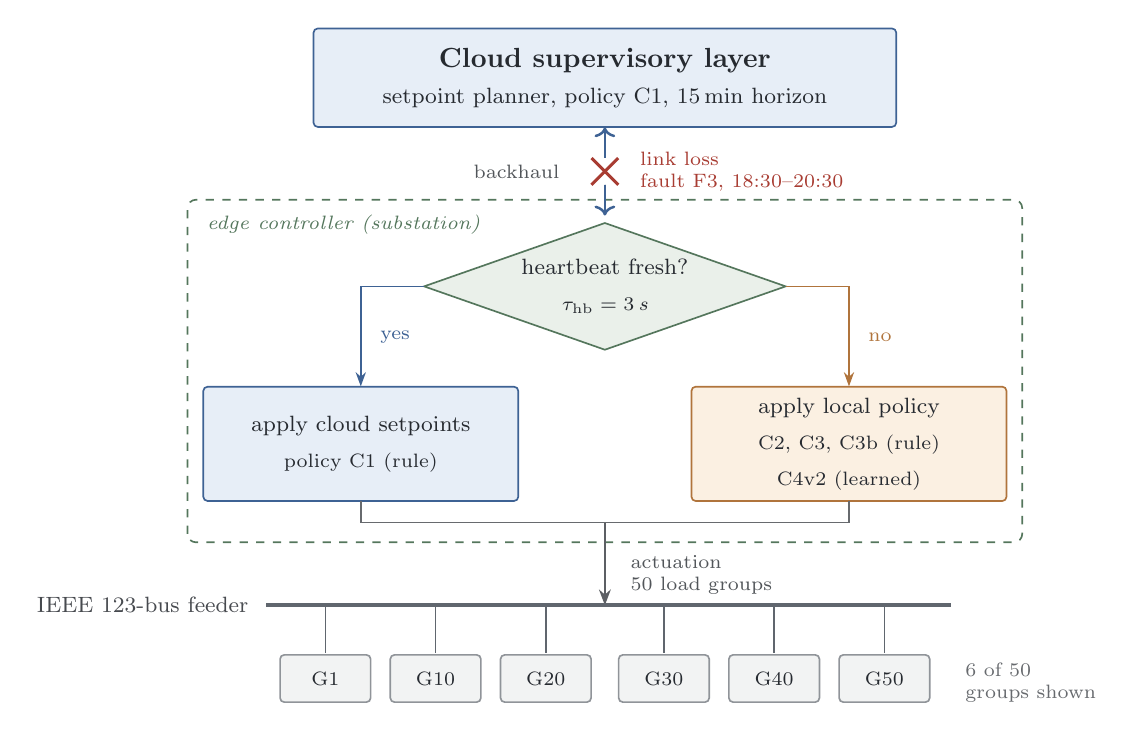
\begin{tikzpicture}[x=1cm, y=1cm, line width=0.6pt, color=ink]

% ============ cloud layer ============
\node[basebox, draw=cloudline, fill=cloudfill,
      minimum width=7.4cm, minimum height=1.25cm] (cloud) at (6.3,9.25)
  {\textbf{Cloud supervisory layer}\\[1pt]
   {\footnotesize setpoint planner, policy C1, 15\,min horizon}};

% ============ backhaul ============
\draw[<->, line width=0.9pt, draw=cloudline] (6.3,8.62) -- (6.3,7.50);
\node[anchor=east, font=\scriptsize, text=ink!80] at (5.85,8.06) {backhaul};

% broken-link marker
\fill[white] (6.3,8.06) circle (0.17);
\draw[faultred, line width=1.1pt] (6.13,7.89) -- (6.47,8.23);
\draw[faultred, line width=1.1pt] (6.13,8.23) -- (6.47,7.89);
\node[anchor=west, font=\scriptsize, text=faultred, align=left]
  at (6.62,8.06) {link loss\\fault F3, 18:30--20:30};

% ============ edge controller ============
\begin{scope}[on background layer]
  \draw[dashed, draw=edgeline, line width=0.6pt, rounded corners=3pt]
    (1.0,3.35) rectangle (11.6,7.70);
\end{scope}
\node[anchor=north west, font=\scriptsize\itshape, text=edgeline]
  at (1.12,7.63) {edge controller (substation)};

% guard diamond
\node[diamond, aspect=2.55, draw=edgeline, fill=edgefill, line width=0.6pt,
      minimum width=4.6cm, inner sep=1pt, align=center] (guard) at (6.3,6.60)
  {\footnotesize heartbeat fresh?\\[1pt]
   \scriptsize\itshape $\tau_{\mathrm{hb}} = 3$\,s};

% ============ policy branches ============
\node[basebox, draw=cloudline, fill=cloudfill,
      minimum width=4.0cm, minimum height=1.45cm] (pcloud) at (3.2,4.60)
  {\footnotesize apply cloud setpoints\\[1pt] \scriptsize policy C1 (rule)};

\node[basebox, draw=localline, fill=localfill,
      minimum width=4.0cm, minimum height=1.45cm] (plocal) at (9.4,4.60)
  {\footnotesize apply local policy\\[1pt]
   \scriptsize C2, C3, C3b (rule)\\[1pt] \scriptsize C4v2 (learned)};

\draw[thinflow, draw=cloudline] (4.0,6.60) -- (3.2,6.60) -- (3.2,5.33);
\draw[thinflow, draw=localline] (8.6,6.60) -- (9.4,6.60) -- (9.4,5.33);
\node[anchor=west, font=\scriptsize, text=cloudline] at (3.32,5.95) {yes};
\node[anchor=west, font=\scriptsize, text=localline] at (9.52,5.95) {no};

% ============ merge to actuation ============
\draw[line width=0.6pt, draw=ink!70] (3.2,3.88) -- (3.2,3.60);
\draw[line width=0.6pt, draw=ink!70] (9.4,3.88) -- (9.4,3.60);
\draw[line width=0.6pt, draw=ink!70] (3.2,3.60) -- (9.4,3.60);
\draw[flow] (6.3,3.60) -- (6.3,2.55);
\node[anchor=west, font=\scriptsize, align=left, text=ink!80]
  at (6.5,2.94) {actuation\\50 load groups};

% ============ feeder ============
\draw[line width=1.4pt, draw=busgrey] (2.0,2.55) -- (10.7,2.55);
\node[anchor=east, font=\footnotesize, text=ink!85] at (1.90,2.55)
  {IEEE 123-bus feeder};

\foreach \x/\lab in {2.75/G1, 4.15/G10, 5.55/G20, 7.05/G30, 8.45/G40, 9.85/G50}{
  \draw[line width=0.6pt, draw=busgrey] (\x,2.55) -- (\x,1.95);
  \node[basebox, draw=busgrey!70, fill=busgrey!8,
        minimum width=1.15cm, minimum height=0.6cm, inner sep=1pt,
        font=\scriptsize] at (\x,1.62) {\lab};
}

% ============ side note ============
\node[anchor=north west, font=\scriptsize, text=ink!70, align=left]
  at (10.75,1.95) {6 of 50\\groups shown};

\end{tikzpicture}
\end{document}
